\pagebreak
\section{Manifolds}
Let's first show some motivation for defining manifolds.
Let's imagine that we have a rectangle cut out of paper that we're trying to fold.
If we fold it and then glue the opposing sides as drawn on the figure, then this will be a torus:

\begin{figure*}[h]
    \centering
    \subfloat{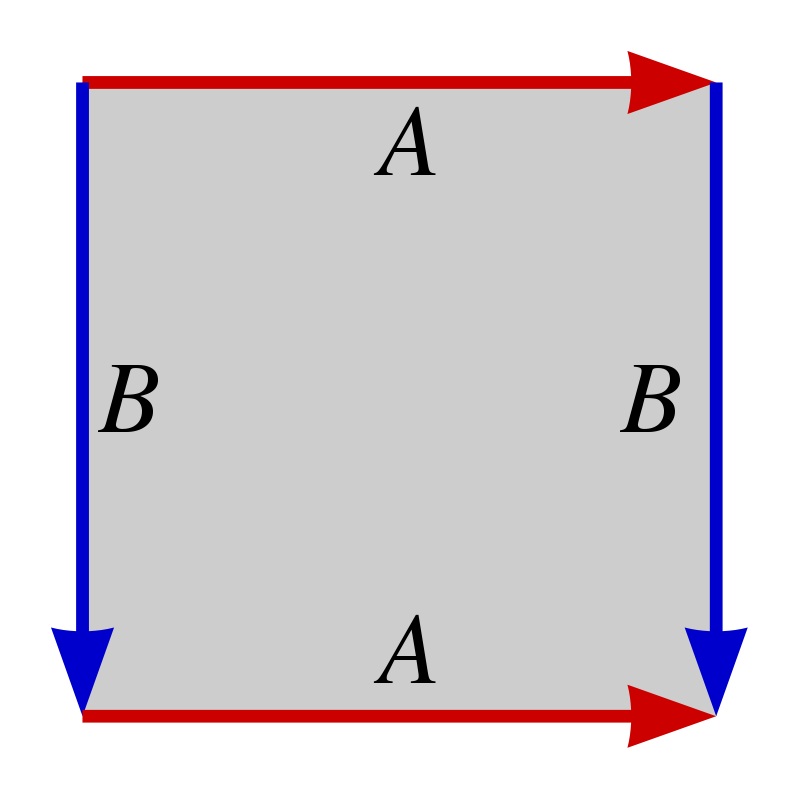
\includegraphics[width=0.2\textwidth]{torus}}
    \qquad
    \subfloat{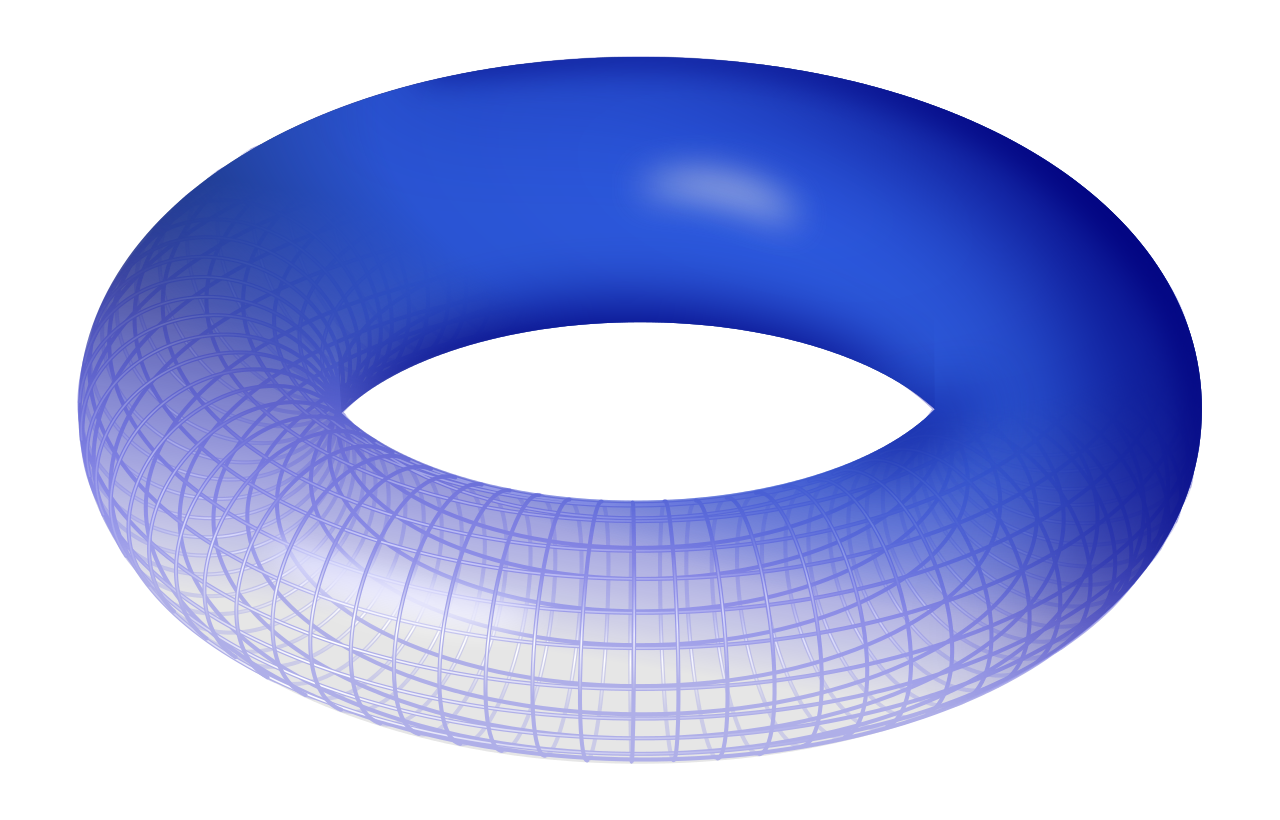
\includegraphics[width=0.2\textwidth]{torus2}}
\end{figure*}

However, it's not obvious whether we can glue the opposing sides like on the next figure.
This is the so-called Klein bottle:

\begin{figure*}[h]
    \centering
    \subfloat{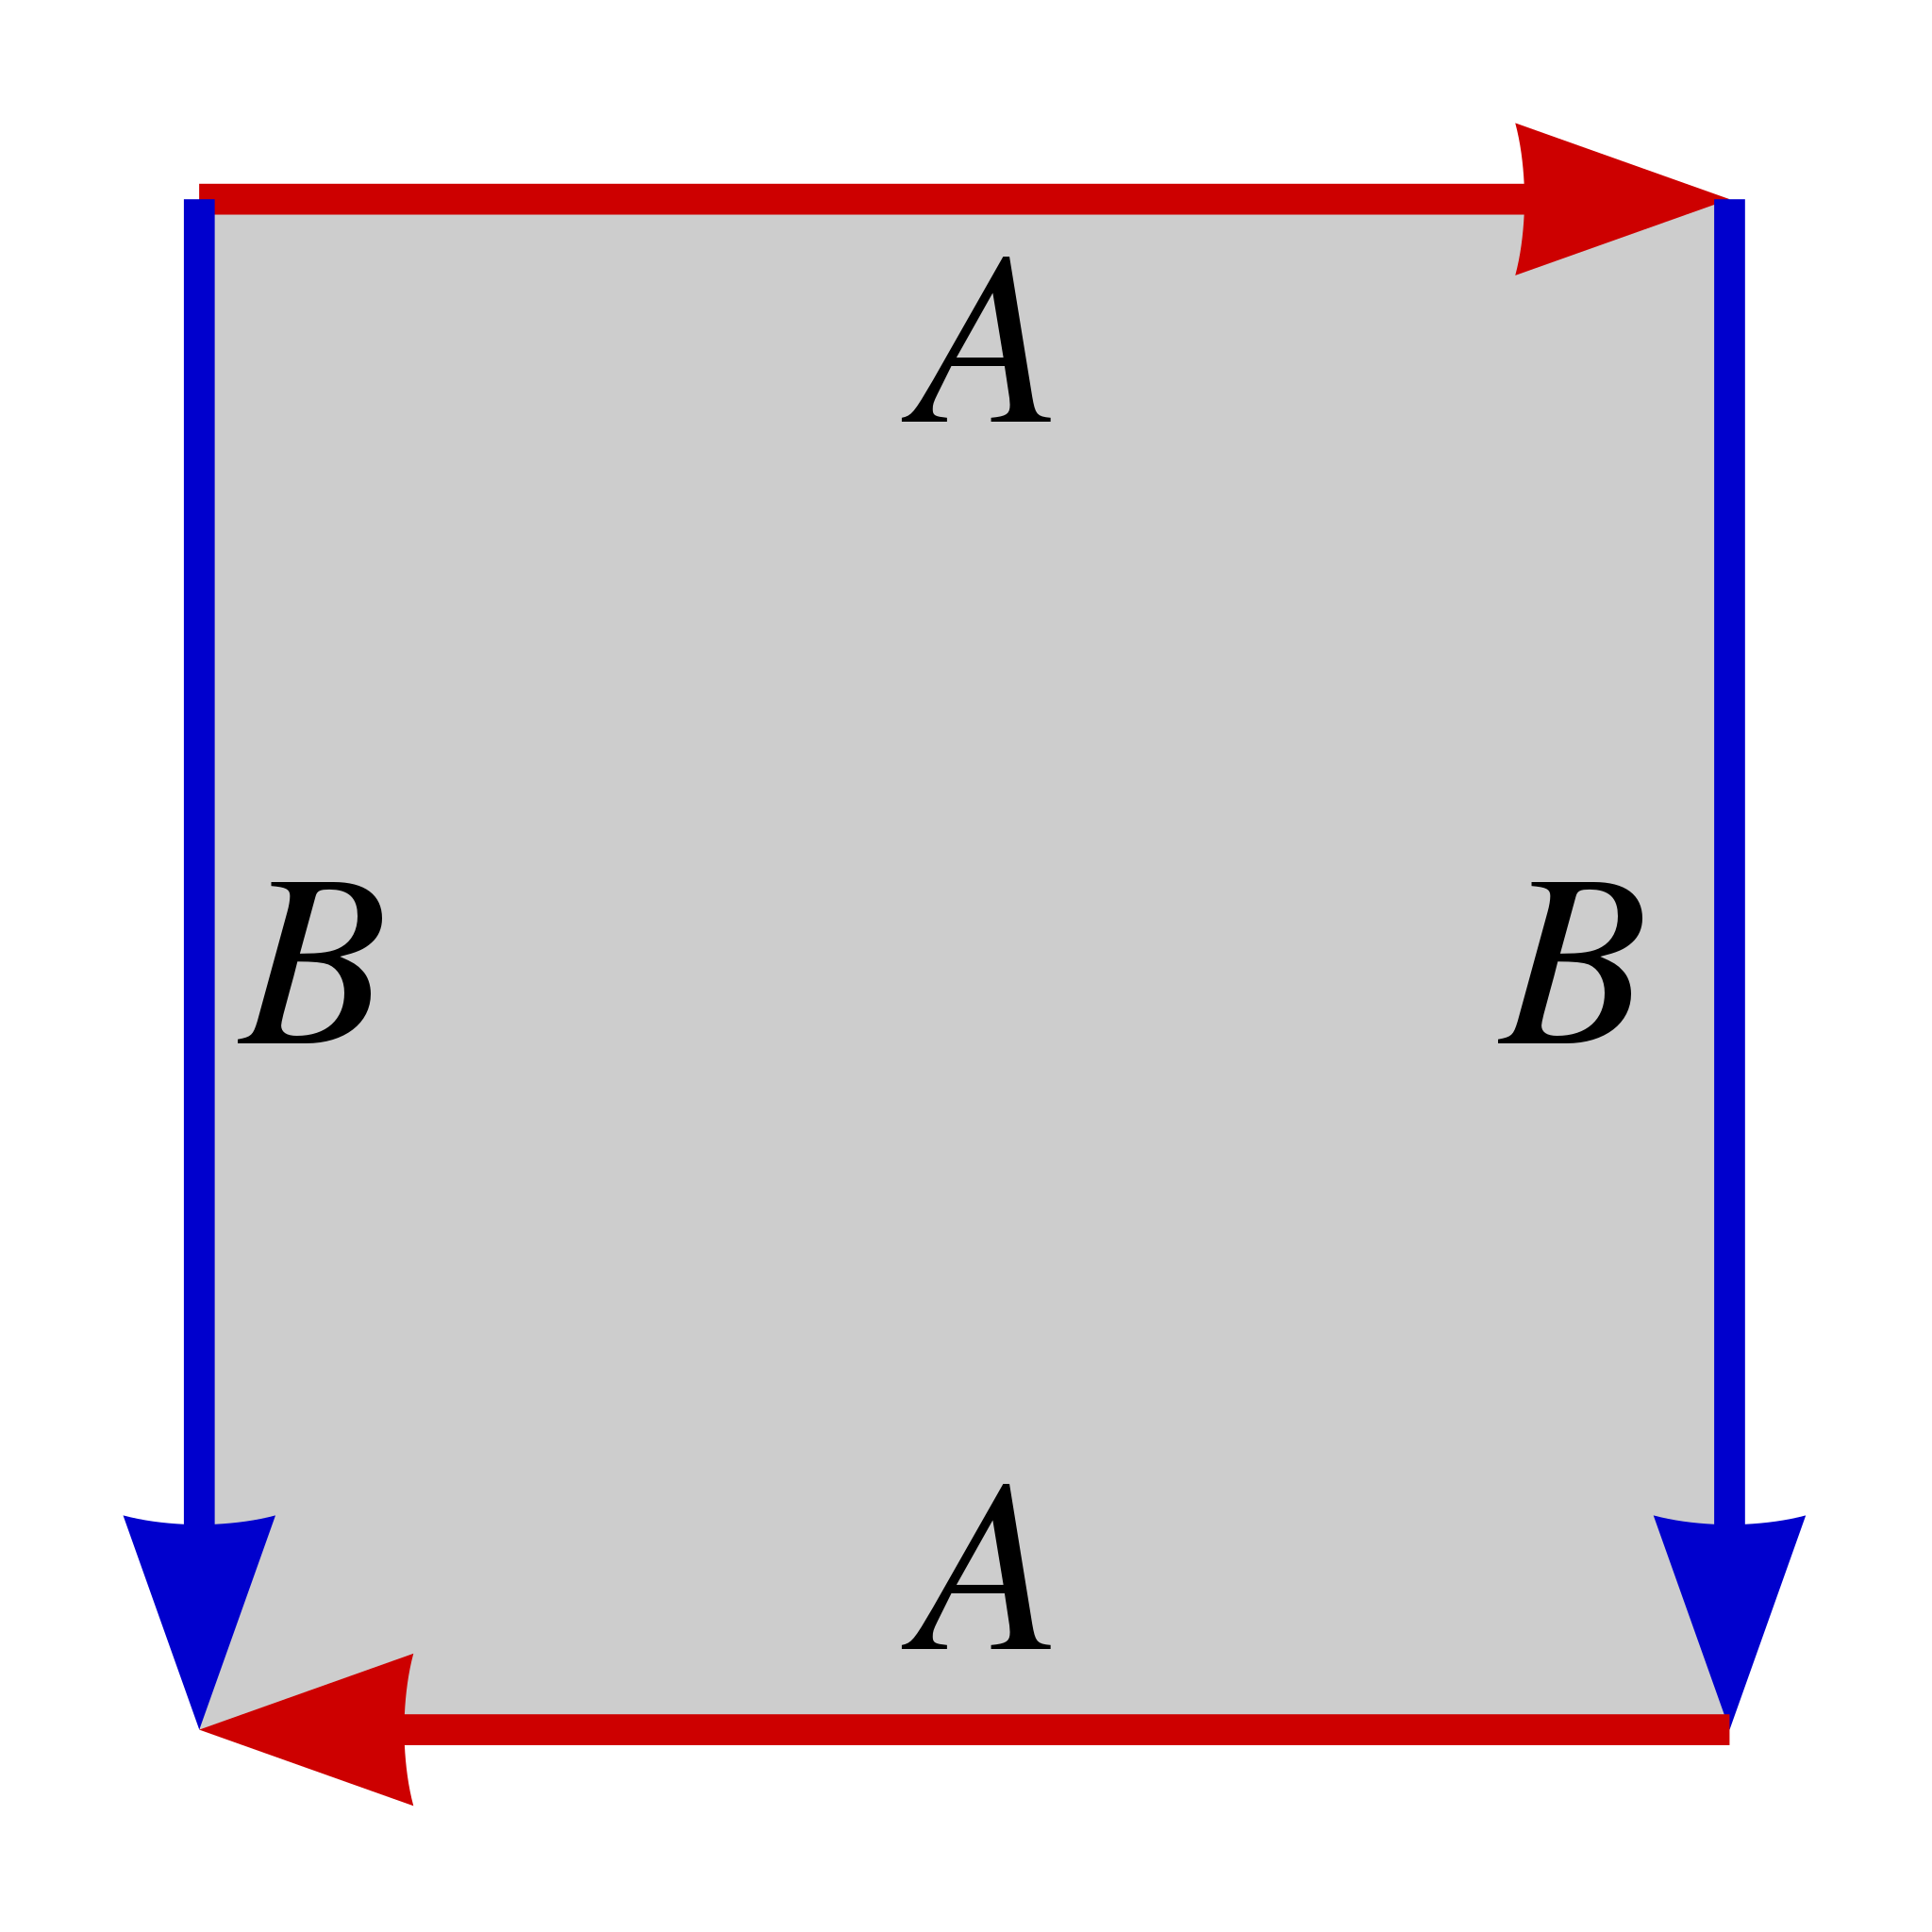
\includegraphics[width=0.2\textwidth]{klein}}
    \qquad
    \subfloat{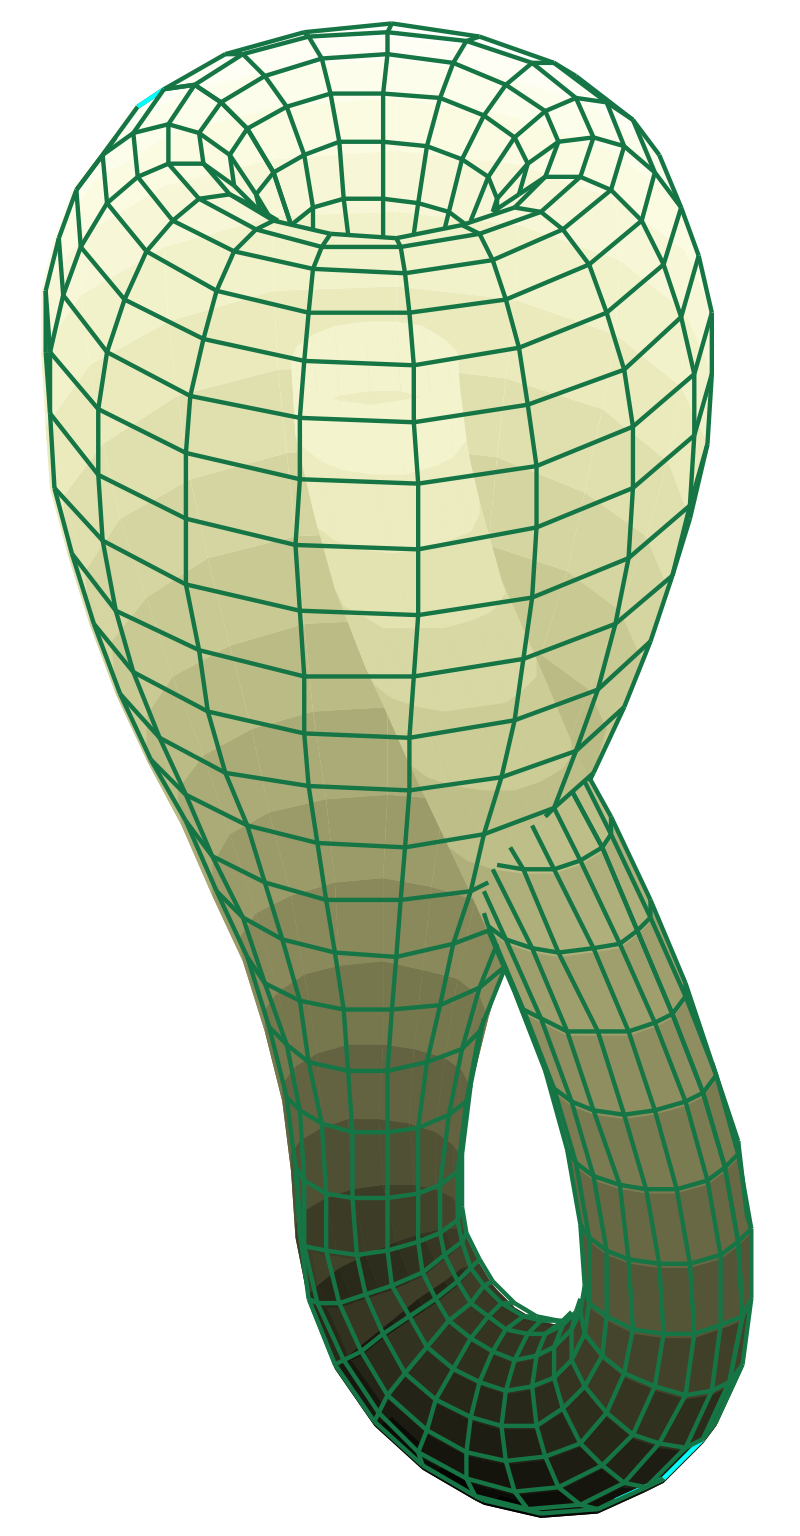
\includegraphics[width=0.13\textwidth]{klein2}}
\end{figure*}

At every point of the surface it looks like $\mathbb{R}^2$!

\subsection{Review of topology}
\begin{definition}[Topological space]
    $X$ --- a set, $\tau = \{U_\alpha \subset X\}_{\alpha \in I}$
    ($I$ --- some index set).
    \begin{enumerate}
        \item {
            $\emptyset, X \in \tau$.
        }
        \item {
            Arbitrary unions of sets from $\tau$ are in $\tau$.
        }
        \item {
            Finite intersections of sets from $\tau$ are in $\tau$.
        }
    \end{enumerate}
    Then $(X, \tau)$ is a \textit{topological space}.
    $U_\alpha$ are called \textit{open sets}. Each $U_\alpha^C$ is a \textit{closed set}.
\end{definition}
\begin{example}
    If $d(\, \cdot\, , \, \cdot \,)$ is a metric on $X$, then 
    $B_r(x) = \{y \in X \mid d(x, y) < r\}$ and $U \subset X$ is open, 
    if $\forall x \in U: \exists r > 0: B_r(x) \subset U$.
\end{example}

A topological space is the smallest structure on a set that allows us to talk about
convergence: a sequence of points in a set converges to a limit, if
for every open set containing this limit the sequence is contained
in that open set starting from some $N$.

\begin{definition}
    $f : X \to Y$ is \textit{continuous} if the preimage of any open set in $Y$
    is open in $X$.
\end{definition}
\begin{definition}
    A bijection $f : X \to Y$ with $f$ and $f^{-1}$ being continuous is called a
    \textit{homeomorphism}.
\end{definition}
\begin{remark}
    Since $f$ is continuous,
    this means that $f^{-1}$ maps every open set in $Y$ to an open set in $X$.
    But since $f^{-1}$ is continuous as well, this means that 
    $f$ maps every open set in $X$ to an open set in $Y$.

    Therefore, $f$ creates a bijection between open sets in $X$ and in $Y$.
\end{remark}
\begin{example}
    \begin{enumerate}
        \item {
            $
                \arctan: (-\infty, +\infty) \to
                \bigl(-\frac{\pi}{2}, \frac{\pi}{2}\bigr)
            $ is a homeomorphism.
        }
        \item {
            \[
                f: [0, 1) \cup [2, 3] \to [0, 2] \qquad
                f(x) = \begin{cases}
                    x & \text{if } x \in [0, 1)\\
                    x - 1 & \text{if } x \in [2, 3]
                \end{cases}
            \]
            Here we have an induced topology on $[0, 1) \cup [2, 3]$. Is this a homeomorphism?
            \begin{enumerate}
                \item {
                    $f$ is a bijection.
                }
                \item {
                    Is $f$ continuous? We need to check that the preimage of an any open 
                    set $U$ in $[0, 2]$ is open in $[0, 1) \cup [2, 3]$.
                    Part of the preimage will be mapped into $[0, 1)$, and part
                    will be mapped into $[2, 3]$.
                    
                    It can be shown that the left endpoint of $f^{-1}(U \cap [0, 1))$
                    and the right endpoint of $f^{-1}(U \cap [1, 2])$ will be excluded.
                    Therefore, the preimage in question can be represented as
                    \[
                        \bigl(f^{-1}(U \cap [0, 1)),\, f^{-1}(U \cap [1, 2])\bigr)
                        \cap \bigl([0, 1) \cup [2, 3]\bigr)
                    \]
                    As this is an intersection of an open set in $\mathbb{R}$ with
                    our set, then it's open in the induced topology.
                }
                \item {
                    $f^{-1}$ is not continuous.
                    Let's take the set $[2, 3]$. It's open in $[0, 1) \cup [2, 3]$
                    by the definition of an induced topology. However,
                    \[
                        (f^{-1})^{-1}([2, 3]) = f([2, 3]) = [1, 2]
                    \]
                    $[1, 2]$ is not open, therefore, $f^{-1}$ is not continuous.
                }
            \end{enumerate}
        }
    \end{enumerate}
\end{example}

\begin{definition}
    A topological space $(X, \tau)$ is called \textit{Hausdorff}
    if for all $x, y \in X,\, x \ne y$ there are open neighborhoods
    $U$ of $x$ and $V$ of $y$, such that $U \cap V = \emptyset$.
\end{definition}
\begin{example}
    Zariski topology on $\mathbb{R}$ or $\mathbb{C}$:
    $U$ is open if and only if $U = \emptyset$ or $X \setminus U$ is finite.

    It is not Hausdorff: there is no way to construct non-overlapping neighborhoods
    of two different points, because every open set is $X$ without a just a finite number of points,
    which will still leave us with a continuum of common points.
\end{example}

\begin{definition}[Basis]
    $X$ --- set, $\mathcal{B}$ --- collection of subsets of $X$, such that:
    \begin{enumerate}
        \item {
            \[ X = \bigcup_{B \in \mathcal{B}} B, \quad \emptyset \in \mathcal{B} \]
        }
        \item {
            For all $B_1,\, B_2 \in \mathcal{B}$ and
            $x \in B_1 \cap B_2$, there exists a $B_3 \in \mathcal{B}$ with 
            $x \in B_3 \subset (B_1 \cap B_2)$.
        }
    \end{enumerate}
    Then the set of all unions of elements of $\mathcal{B}$ is called the topology 
    generated by $B$.

    Such $\mathcal{B}$ is called a \textit{basis} of the topology it generates.
\end{definition}
\begin{proposition}
    The definition is correct, i.e. this is indeed a topology.
\end{proposition}
\begin{proof}
    \begin{enumerate}
        \item {
            $\emptyset,\, X \in \tau$ --- true, because we can
            take the empty union and the union of all $B \in \mathcal{B}$.
        }
        \item {
            Unions of $U_\alpha$'s from $\tau$ are in $\tau$ --- we can 
            just take the union of the corresponding elements from $\mathcal{B}$.
        }
        \item {
            Let's prove that the intersection of two open sets $U_\alpha$ and $U_\beta$
            is open, then use induction to prove that for finite intersections.

            Let's assume $x \in U_\alpha \cap U_\beta$.
            Since $U_\alpha$ is a union of sets from $\mathcal{B}$, we can 
            choose the one that contains $x$ and call it $B_1$. Let's do the same thing with
            $U_\beta$ and $B_2$. So,
            $x \in B_1 \cap B_2$ where $B_1 \subset U_1,\ B_2 \subset U_\beta$.

            By the definition of $\mathcal{B}$, there exists a
            $B_{3,x} \subset U_\alpha \cap U_\beta$, such that $x \in B_{3,x}$.
            $B_{3,x}$ is open, because it's a union of just one set from $\mathcal{B}$.
            Since $x \in U_\alpha \cap U_\beta$ was arbitrary,
            \[
                U_\alpha \cap U_\beta = \bigcup_{x \in U_\alpha \cap U_\beta} B_{3, x}
            \]
            Therefore, $U_\alpha \cap U_\beta$ as a union of open sets. 
        }
    \end{enumerate}
\end{proof}

\begin{definition}
    A topological space is called \textit{second-countable} if it has a countable basis.
\end{definition}

\begin{proposition}
    Second-countability implies
    \hyperref[def:separable]{separability}.
\end{proposition}
\begin{proof}
    Let's assume we have a second-countable set with a countable basis $\mathcal{B}$.
    Choose an arbitrary point in each element of $\mathcal{B}$ to form
    a countable set in $A$. If $A$ is not dense,
    then there exists an open set $U$, such that $U \cap A = \emptyset$.
    But since $\mathcal{B}$ is a basis, $U$ is some union of elements of 
    $\mathcal{B}$. Let's take one of those elements, $B_U$.
    We've chosen a point $x$ in $B_U$:
    \[
        \begin{cases}
            x \in B_U \subset U\\
            x \in A
        \end{cases} \implies
        x \in U \cap A \implies U \cap A \ne \emptyset \text{?!}
    \]
\end{proof}
\begin{remark}
    The inverse is not true: there are separable sets that are not second-countable.
\end{remark}

\begin{definition}
    $M$ is a \textit{topological manifold of dimension $n$}
    if it is a Hausdorff and second-countable topological space, such that
    every point in $M$ has a neighborhood homeomorphic to an open set in
    $\mathbb{R}^n$.

    (For all $p \in M$ there exists an open $U \subset M$,
    such that $p \in U$ and there exist an open $V \in \mathbb{R}^n$ and
    a homeomorphism $\varphi : U \to V$.)
\end{definition}
\begin{remark}
    This definition would work for a Klein bottle. Locally around every point
    it looks like a plane.
\end{remark}
\begin{remark}
    It turns out that the number $n$ is a topological invariant, i.e.
    two topological manifolds cannot be homeomorphic if their dimensions differ.
    
    Exercise: reduce this to the following statement:
\end{remark}
\begin{theorem}[Brower's invariance of domain]
    Let $U \subset \mathbb{R}^n$ be open, and let $f : U \to \mathbb{R}^n$
    be continuous and injective. Then $f(U)$ is open in $\mathbb{R}^n$.
\end{theorem}
We're not gonna prove this theorem.
Let's look at a simpler case: a continuous injective function in $\mathbb{R}$.
$f : \mathbb{R} \to \mathbb{R}$. If $f \in C^1(\mathbb{R})$, then
\[ f(x) = f(x_0) + f'(x_0)(x - x_0) + o(\abs{x - x_0}) \]
If $f'(x_0)$ is not zero,
it follows that $f(x_0)$ cannot be a boundary point, since 
$ f(x) - f(x_0)$ will have two different signs around $x_0$.
But again, $f'(x_0)$ can have zeros, so this is not a full proof.

\begin{samepage}
\begin{definition}
    A pair $(U, \varphi)$ with $U \subset M$ --- an open set and
    $\varphi: U \to \mathbb{R}^n$ --- a homeomorphism from
    $U$ to $\varphi(U) = V$ is called a \textit{chart}.
    \begin{itemize}
        \item {
            $\varphi$ is a local coordinate map.
        }
        \item {
            $\varphi(p) = \bigl(x^1(p), x^2(p), \dots, x^n(p)\bigr)$ --- local
            coordinates. They don't work on the whole $M$ --- just on $U$.
        }
        \item {
            $\varphi^{-1} : V \to U$ is called a \textit{coordinate system}.
        }
    \end{itemize}
\end{definition}
\end{samepage}
Examples of topological manifolds:
\begin{enumerate}
    \item {
        An open set in $\mathbb{R}^n$. We only need one chart --- $\mathbb{R}^n$ itself.
    }
    \item {
        The $n$-sphere 
        \[
             S^n \coloneqq \{ (x^1, \dots, x^{n+1}) \in \mathbb{R}^{n+1}
             \mid {\textstyle \sum} (x^j)^2 = 1 \} 
        \]
        We would need two charts. Let's have one chart as
        the sphere except the north pole with homeomorphism as a stereographic projection,
        and the other as the sphere except the south pole.
        The two charts overlap, but they still satisfy the definition.

        \begin{figure*}[h]
            \centering
            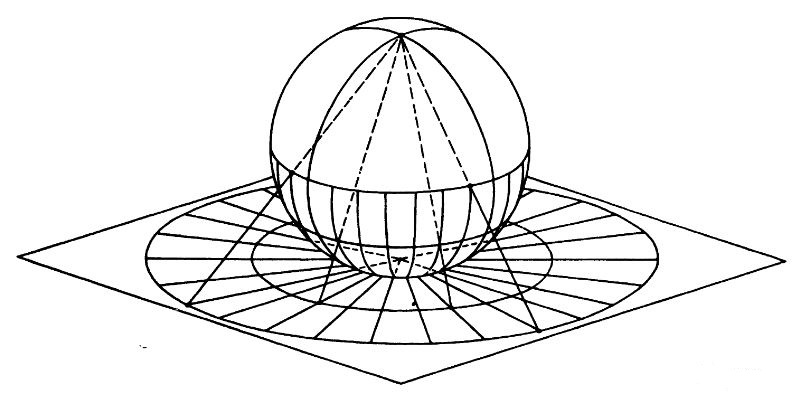
\includegraphics[width=0.4\textwidth]{stereographic}
        \end{figure*}
    }
    \item {
        $\mathbb{P}^n$ --- projective space.
        $\mathbb{P}^n = \bigl(\mathbb{R}^n \setminus \{0\} \bigr) / \sim$.
        (We're gonna define $\sim$ later).

        $\mathbb{P}^1$ --- the set of all lines in $\mathbb{R}^2$ passing through
        the origin:
        \begin{center}   
            \begin{tikzpicture}
                \begin{axis}[
                    axis x line=center,
                    axis y line=center,
                    axis line style={-{Stealth[scale=1.5]}},
                    ytick={1},
                    xtick=\empty,
                    xmin=-2, xmax=2, ymin=-1, ymax=2,
                    unit vector ratio=1 1 1,
                    samples=100,
                ]
                    \tikzset{graph/.style={very thick, smooth, domain=-2:2}}
                    \tikzset{graph_point/.style={fill,circle,inner sep=1.5pt}}
                    \addplot[red, graph] {1};
                    \addplot[blue, graph] {x};
                    \addplot[blue, graph] {-x};
                    \addplot[blue, graph] {2 * x};
                    \addplot[blue, graph] {-2 * x};
                    \node[graph_point] at (1, 1){};
                    \node[graph_point] at (0.5, 1){};
                    \node[graph_point] at (-0.5, 1){};
                    \node[graph_point] at (-1, 1){};
                \end{axis}
            \end{tikzpicture}
        \end{center}
        Every non-horizontal line passing through the origin can be mapped onto 
        a point on the red line. A horizontal line corresponds to the 
        point at infinity. So, essentially, $\mathbb{P}^1$ 
        is equivalent the `extended 'real line. 

        Here's how we're gonna define our equivalence relation:
        $(x_1, y_1) \sim (x_2, y_2)$ if and only if $x_1 = kx_2$ and $y_1 = ky_2$,
        i.e. if they're on the same line:
        \begin{center}   
            \begin{tikzpicture}
                \begin{axis}[
                    axis x line=center,
                    axis y line=center,
                    axis line style={-{Stealth[scale=1.5]}},
                    ytick={1},
                    xtick=\empty,
                    xmin=-1, xmax=3, ymin=-1, ymax=2.5,
                    unit vector ratio=1 1 1,
                    samples=100,
                ]
                    \tikzset{graph/.style={very thick, smooth, domain=-1:2.7}}
                    \tikzset{graph_point/.style={fill,circle,inner sep=1.5pt}}
                    \addplot[red, graph] {1};
                    \addplot[blue, graph] {x};
                    \node[graph_point] at (1, 1){};
                    \node[graph_point,label=0:{$(x_2, y_2)$}] at (1.5, 1.5){};
                    \node[graph_point,label=0:{$(x_1, y_1)$}] at (2, 2){};
                \end{axis}
            \end{tikzpicture}
        \end{center}
        This equivalence relation can be exteneded to $\mathbb{R}^{n+1}$.

        Now, here's how we're gonna define the charts.
        $p \in \mathbb{P}^n \implies$ take a representative
        $(x_1, \dots, x_{n+1})$. Choose $x_i \ne 0$.
        Without the loss of generality, $i = n + 1$, therefore, in some
        neighborhood $U$ around $p$ we have $x_{n + 1} \ne 0$.
        For each point in $U$:
        \[
            \Bigl(\frac{y_1}{y_{n+1}}, \frac{y_2}{y_{n+1}}, \dots, \frac{y_n}{y_{n - 1}}, 1\Bigr)
            \sim (y_1, \dots, y_{n + 1})
        \]
        So, around every point of the projective space we can find a chart:
        take any representative of that point, find a non-zero coordinate.
        This coordinate will remain non-zero in some neighborhood, therefore,
        we can divide by it, and this coordinate by which we divide 
        will turn to $1$. The remaining $n$ coordinates will define the coordinates of a point
        in $\mathbb{R}^n$, which will provide a local homeomorphism around
        the point in the projective space to a subset $\mathbb{R}^n$, 
        which defines a chart.
    }
\end{enumerate}